A study was carried out to choose the length of scintillating fibers that optimize the tritium detection efficiency. For this task, the complete TRITIUM-Aveiro prototype was simulated, in which the photon propagation was included.

First, the propagation of photons in scintillating fibers was studied. The blue distribution of Figure \ref{fig:PhotonsFibersYesNoPhotosensors} shows the number of photons produced in the fiber per tritium event that reaches them and the red distribution shows the same information but only for those events detected for both photosensors in time coincidence.

\begin{figure}[h]
\centering
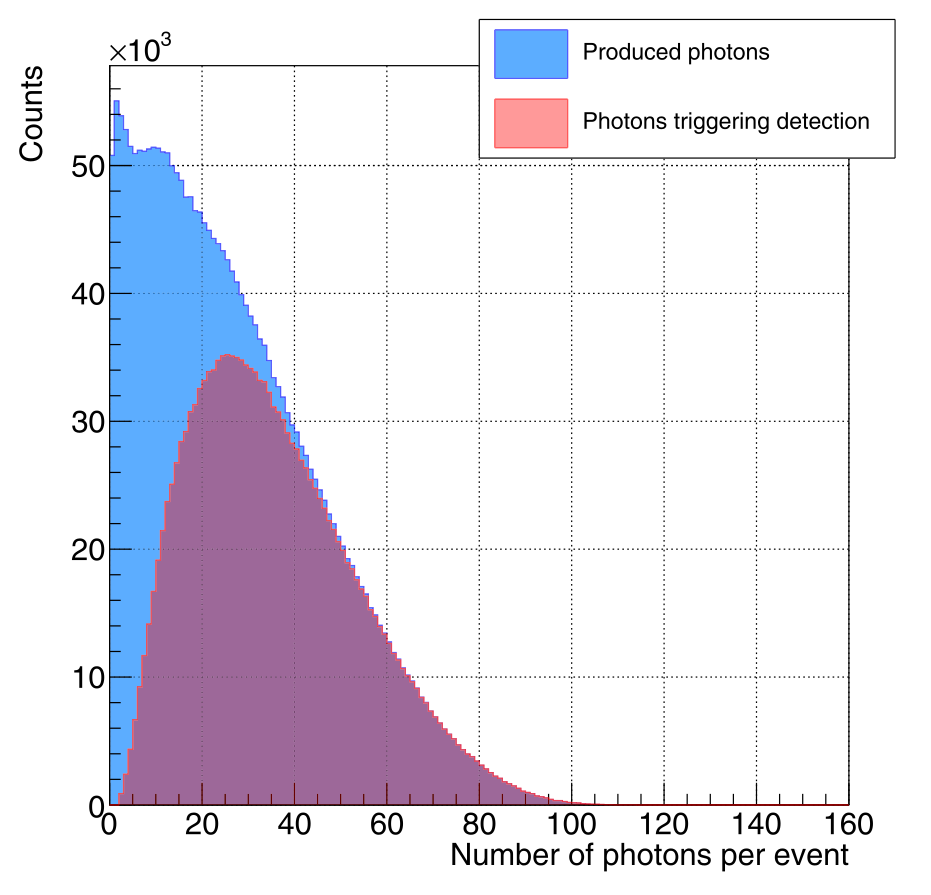
\includegraphics[scale=0.3]{Figures/8SimulationsResults/81TRITIUMDesign/813Length/CollectionPhotonsInFibers.png}
\caption{Number of photons produced in the fiber per tritium event for all tritium events that reach the fiber (blue histogram) and only for tritium events the photons of which are detected by photosensors (red histogram) \cite{SimulationPaperCarlos}.\label{fig:PhotonsFibersYesNoPhotosensors}}
\end{figure}

It can be seen that tritium events that produce a high number of photons are practically always detected but most of the events with fewer photons produced in the fibers are not detected, producing a peak centred of around $25$ photons.  

Regarding the fiber length study, two different lengths were compared, $1~\meter$ and $0.20~\meter$, and two different tritium source activity were used, $0.5~\kilo\becquerel/\liter$ and $2.5~\kilo\becquerel/\liter$. As detected tritium counts is proportional to the active area, 5 detectors were simulated for the case of $0.20~\meter$ fiber length to normalize the study to the same active area. The counts, which were integred over $60~\min$ and taken over a week, are shown in Figure \ref{fig:CountsOver60minDifferentLength}.

\begin{figure}[h]
\centering
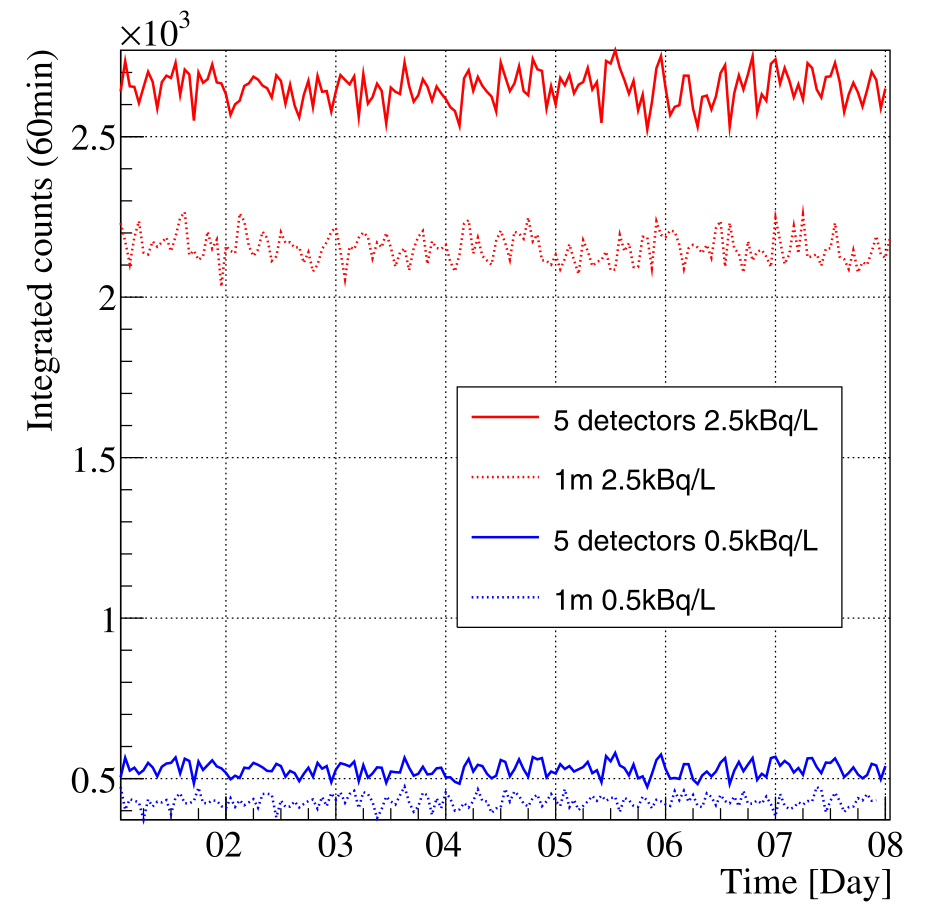
\includegraphics[scale=0.3]{Figures/8SimulationsResults/81TRITIUMDesign/813Length/2DifferentLength.png}
\caption{Counts integred over $60~\min$, normalized to the same active area and taken over a week for a fiber length of $1~\meter$, dashed lines, and $20~\cm$, solid lines and two different activities, $0.5~\kilo\becquerel/\liter$, blue lines, and $2.5~\kilo\becquerel/\liter$, red lines \cite{SimulationPaperCarlos}. \label{fig:CountsOver60minDifferentLength}}
\end{figure}

A larger signal is seen for shorter fiber lengths in both cases, producing a increasement in tritium detection efficiency of approximately $25\%$, principally caused by a lower absortion of photons in shorter scintillating fibers and the leakage of some photons due to a non-perfect photon collection in the fiber.